\documentclass[12pt,letterpaper]{hmcpset}
\usepackage[margin=1in]{geometry}
\usepackage{graphicx}
\usepackage[makeroom]{cancel}
\usepackage{array}
\usepackage{mathtools}
\usepackage{marginnote}
\usepackage{units}
\usepackage{xfrac}
\usepackage{enumerate}
\usepackage{amsmath}
\usepackage{fancyhdr}
\usepackage{pgfplots}
\usepackage{hyperref}
\usepackage{nopageno}
\hypersetup{
	colorlinks=true,
	linkcolor=blue,
	filecolor=magenta,      
	urlcolor=magenta,
}

% info for header block in upper right hand corner
\name{} %put your name here
\class{Physics 51 Section \hspace{3mm}} %put your section here
\assignment{Homework 7}
\duedate{Monday, October 12, 2020}

\begin{document}
	\begin{problem}[33P12:]
		A conductor consists of an infinite number of adjacent wires, each infinitely long carrying a current $i$.
		Show that the lines of $\vec{\mathbf{B}}$ are as represented in Fig. 33-61 and that $B$ for all points above and below the infinite current sheet is given by
		\[B = \frac{1}{2}\mu_0ni,\]
		where $n$ is the number of wires per unit length.
		Derive both by direct application of Ampère's law and by considering the problem as a limiting case of Sample Problem 33-5.

		\centering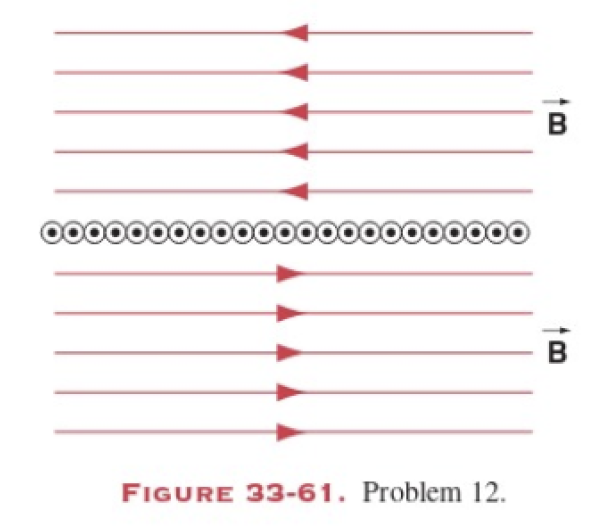
\includegraphics[scale = 0.4]{Fig_33-61}
	\end{problem}
	\clearpage



	\begin{problem}[33P13:]
		The current density inside a long, solid, cylindrical wire of radius $a$ is in the direction of the axis and varies linearly with radial distance $r$ from the axis according to $j = j_0\frac{r}{a}$.
		Find the magnetic field inside the wire.
		Express your answer in terms of the total current $i$ carried by the wire.
	\end{problem}
	\clearpage



	\begin{problem}[34E26:]
		A stiff wire bent into a semicircle of radius $a$ is rotated with a frequency $f$ in a uniform magnetic field, as suggested in Fig. 34-51.
		What are $(a)$ the frequency and $(b)$ the amplitude of the emf induced in the loop?

		\centering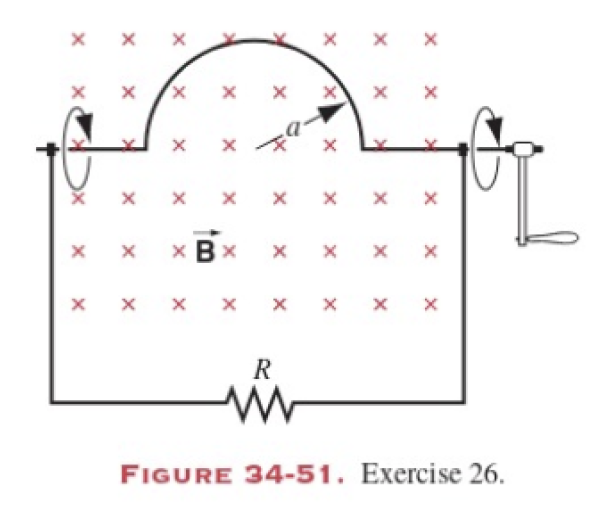
\includegraphics[scale = 0.4]{Fig_34-51}
	\end{problem}
	\clearpage



	\begin{problem}[34E23:]
	A rectangular loop of wire with length $a$, width $b$, and resistance $R$ is placed near an infinitely long wire carrying current $i$, as shown in Fig. 34-49.
		The distance from the long wire to the loop is $D$.
		Find $(a)$ the magnitude of the magnetic flux through the loop and $(b)$ the current in the loop as it moves away from the long wire with speed $v$.

		\centering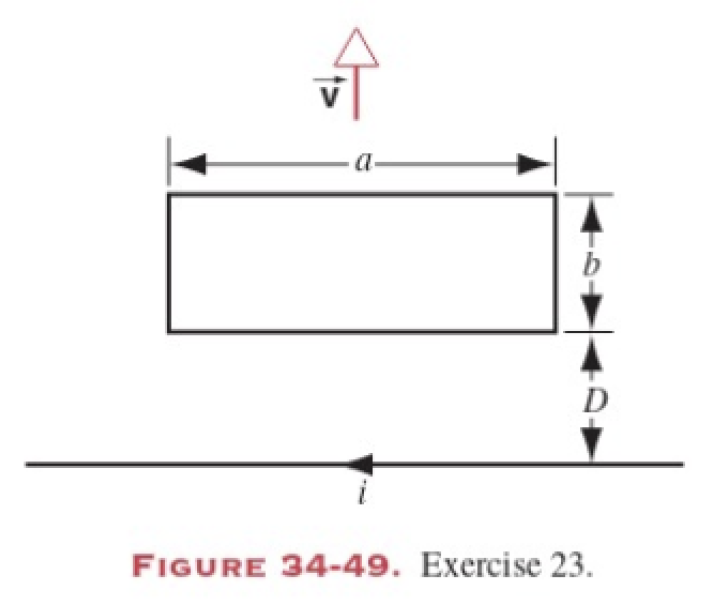
\includegraphics[scale = 0.3]{Fig_34-49}
	\end{problem}
	\clearpage



	\begin{problem}[34P9:]
		A rod with length $L$, mass $m$, and resistance $R$ slides without friction down parallel conducting rails of negligible resistance, as in Fig. 34-59.
		The rails are connected together at the bottom as shown, forming a conducting loop with the rod as the top member.
		The plane of the rails makes an angle $\theta$ with the horizontal, and a uniform vertical magnetic field $\vec{\mathbf{B}}$ exists throughout the region.

		\centering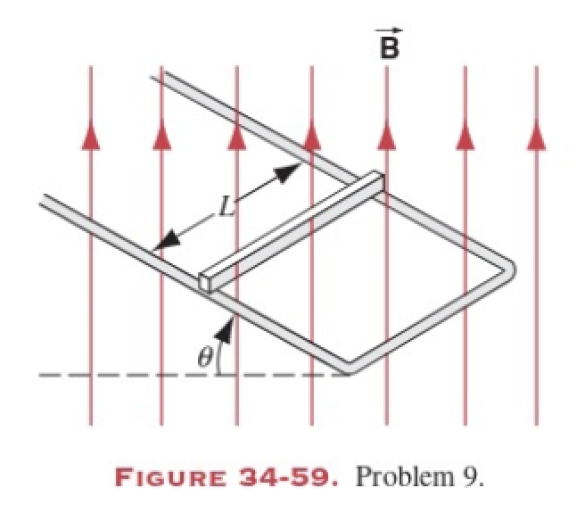
\includegraphics[scale = 0.4]{Fig_34-59}

		\begin{enumerate}[(a)]
		\item Show that the rod acquires a steady-state terminal velocity whose magnitude is
		\[v = \frac{mgR}{B^2L^2}\frac{\sin{\theta}}{\cos^2{\theta}}.\]
		\item Show that the rate at which the internal energy of the rod is increasing is equal to the rate at which the rod is losing gravitational potential energy.
		\item Discuss the situation if $\vec{\mathbf{B}}$ were directed downward instead of up.
		\end{enumerate}
	\end{problem}
	\clearpage



	\begin{problem}[34E30:]
		A long solenoid has a diameter of 12.6 cm.
		When a current $i$ is passed through its windings, a uniform magnetic field $B$ = 28.6 mT is produced in its interior.
		By decreasing $i$, the field is caused to decrease at the rate 6.51 mT/s.
		Calculate the magnitude of the induced electric field $(a)$ 2.20 cm and $(b)$ 8.20 cm from the axis of the solenoid.
	\end{problem}
	\clearpage
\end{document}
